\documentclass{ximera}

%\usepackage{todonotes}

\newcommand{\todo}{}

\usepackage{tkz-euclide}
\tikzset{>=stealth} %% cool arrow head
\tikzset{shorten <>/.style={ shorten >=#1, shorten <=#1 } } %% allows shorter vectors

\usepackage{tkz-tab}  %% sign charts
\usetikzlibrary{decorations.pathreplacing} 

\usetikzlibrary{backgrounds} %% for boxes around graphs
\usetikzlibrary{shapes,positioning}  %% Clouds and stars
\usetikzlibrary{matrix} %% for matrix
\usepgfplotslibrary{polar} %% for polar plots
\usetkzobj{all}
\usepackage[makeroom]{cancel} %% for strike outs
%\usepackage{mathtools} %% for pretty underbrace % Breaks Ximera
\usepackage{multicol}

\usepackage{polynom}



\usepackage[many]{tcolorbox}  %% for titled boxes
\newtcolorbox{xbox}[1]{%
    tikznode boxed title,
    enhanced,
    arc=0mm,
    interior style={white},
    attach boxed title to top center= {yshift=-\tcboxedtitleheight/2},
    fonttitle=\bfseries,
    colbacktitle=white,coltitle=black,
    boxed title style={size=normal,colframe=white,boxrule=0pt},
    title={#1}}


\usepackage{array}
\setlength{\extrarowheight}{+.1cm}   
\newdimen\digitwidth
\settowidth\digitwidth{9}
\def\divrule#1#2{
\noalign{\moveright#1\digitwidth
\vbox{\hrule width#2\digitwidth}}}





\newcommand{\RR}{\mathbb R}
\newcommand{\R}{\mathbb R}
\newcommand{\N}{\mathbb N}
\newcommand{\Z}{\mathbb Z}

%\renewcommand{\d}{\,d\!}
\renewcommand{\d}{\mathop{}\!d}
\newcommand{\dd}[2][]{\frac{\d #1}{\d #2}}
\newcommand{\pp}[2][]{\frac{\partial #1}{\partial #2}}
\renewcommand{\l}{\ell}
\newcommand{\ddx}{\frac{d}{\d x}}
\newcommand{\ddt}{\frac{d}{\d t}}

\newcommand{\zeroOverZero}{\ensuremath{\boldsymbol{\tfrac{0}{0}}}}
\newcommand{\inftyOverInfty}{\ensuremath{\boldsymbol{\tfrac{\infty}{\infty}}}}
\newcommand{\zeroOverInfty}{\ensuremath{\boldsymbol{\tfrac{0}{\infty}}}}
\newcommand{\zeroTimesInfty}{\ensuremath{\small\boldsymbol{0\cdot \infty}}}
\newcommand{\inftyMinusInfty}{\ensuremath{\small\boldsymbol{\infty - \infty}}}
\newcommand{\oneToInfty}{\ensuremath{\boldsymbol{1^\infty}}}
\newcommand{\zeroToZero}{\ensuremath{\boldsymbol{0^0}}}
\newcommand{\inftyToZero}{\ensuremath{\boldsymbol{\infty^0}}}



\newcommand{\numOverZero}{\ensuremath{\boldsymbol{\tfrac{\#}{0}}}}
\newcommand{\dfn}{\textbf}
%\newcommand{\unit}{\,\mathrm}
\newcommand{\unit}{\mathop{}\!\mathrm}
\newcommand{\eval}[1]{\bigg[ #1 \bigg]}
\newcommand{\seq}[1]{\left( #1 \right)}
\renewcommand{\epsilon}{\varepsilon}
\renewcommand{\iff}{\Leftrightarrow}

\DeclareMathOperator{\arccot}{arccot}
\DeclareMathOperator{\arcsec}{arcsec}
\DeclareMathOperator{\arccsc}{arccsc}
\DeclareMathOperator{\si}{Si}
\DeclareMathOperator{\proj}{proj}
\DeclareMathOperator{\scal}{scal}


\newcommand{\tightoverset}[2]{% for arrow vec
  \mathop{#2}\limits^{\vbox to -.5ex{\kern-0.75ex\hbox{$#1$}\vss}}}
\newcommand{\arrowvec}[1]{\tightoverset{\scriptstyle\rightharpoonup}{#1}}
\renewcommand{\vec}{\mathbf}
\newcommand{\veci}{\vec{i}}
\newcommand{\vecj}{\vec{j}}
\newcommand{\veck}{\vec{k}}
\newcommand{\vecl}{\boldsymbol{\l}}

\newcommand{\dotp}{\bullet}
\newcommand{\cross}{\boldsymbol\times}
\newcommand{\grad}{\boldsymbol\nabla}
\newcommand{\divergence}{\grad\dotp}
\newcommand{\curl}{\grad\cross}
%\DeclareMathOperator{\divergence}{divergence}
%\DeclareMathOperator{\curl}[1]{\grad\cross #1}


\colorlet{textColor}{black} 
\colorlet{background}{white}
\colorlet{penColor}{blue!50!black} % Color of a curve in a plot
\colorlet{penColor2}{red!50!black}% Color of a curve in a plot
\colorlet{penColor3}{red!50!blue} % Color of a curve in a plot
\colorlet{penColor4}{green!50!black} % Color of a curve in a plot
\colorlet{penColor5}{orange!80!black} % Color of a curve in a plot
\colorlet{fill1}{penColor!20} % Color of fill in a plot
\colorlet{fill2}{penColor2!20} % Color of fill in a plot
\colorlet{fillp}{fill1} % Color of positive area
\colorlet{filln}{penColor2!20} % Color of negative area
\colorlet{fill3}{penColor3!20} % Fill
\colorlet{fill4}{penColor4!20} % Fill
\colorlet{fill5}{penColor5!20} % Fill
\colorlet{gridColor}{gray!50} % Color of grid in a plot

\newcommand{\surfaceColor}{violet}
\newcommand{\surfaceColorTwo}{redyellow}
\newcommand{\sliceColor}{greenyellow}




\pgfmathdeclarefunction{gauss}{2}{% gives gaussian
  \pgfmathparse{1/(#2*sqrt(2*pi))*exp(-((x-#1)^2)/(2*#2^2))}%
}


%%%%%%%%%%%%%
%% Vectors
%%%%%%%%%%%%%

%% Simple horiz vectors
\renewcommand{\vector}[1]{\left\langle #1\right\rangle}


%% %% Complex Horiz Vectors with angle brackets
%% \makeatletter
%% \renewcommand{\vector}[2][ , ]{\left\langle%
%%   \def\nextitem{\def\nextitem{#1}}%
%%   \@for \el:=#2\do{\nextitem\el}\right\rangle%
%% }
%% \makeatother

%% %% Vertical Vectors
%% \def\vector#1{\begin{bmatrix}\vecListA#1,,\end{bmatrix}}
%% \def\vecListA#1,{\if,#1,\else #1\cr \expandafter \vecListA \fi}

%%%%%%%%%%%%%
%% End of vectors
%%%%%%%%%%%%%

%\newcommand{\fullwidth}{}
%\newcommand{\normalwidth}{}



%% makes a snazzy t-chart for evaluating functions
%\newenvironment{tchart}{\rowcolors{2}{}{background!90!textColor}\array}{\endarray}

%%This is to help with formatting on future title pages.
\newenvironment{sectionOutcomes}{}{} 



%% Flowchart stuff
%\tikzstyle{startstop} = [rectangle, rounded corners, minimum width=3cm, minimum height=1cm,text centered, draw=black]
%\tikzstyle{question} = [rectangle, minimum width=3cm, minimum height=1cm, text centered, draw=black]
%\tikzstyle{decision} = [trapezium, trapezium left angle=70, trapezium right angle=110, minimum width=3cm, minimum height=1cm, text centered, draw=black]
%\tikzstyle{question} = [rectangle, rounded corners, minimum width=3cm, minimum height=1cm,text centered, draw=black]
%\tikzstyle{process} = [rectangle, minimum width=3cm, minimum height=1cm, text centered, draw=black]
%\tikzstyle{decision} = [trapezium, trapezium left angle=70, trapezium right angle=110, minimum width=3cm, minimum height=1cm, text centered, draw=black]


\author{Nela Lakos}

\outcome{Global extrema from a graph.}
\outcome{Extreme value theorem.}


\begin{document}


\begin{exercise}
  Let $f$ be a function defined on $[0,4]$. The graph of $f$ is given in the figure below.
 Based on the graph, answer the questions below.
  \begin{image}
  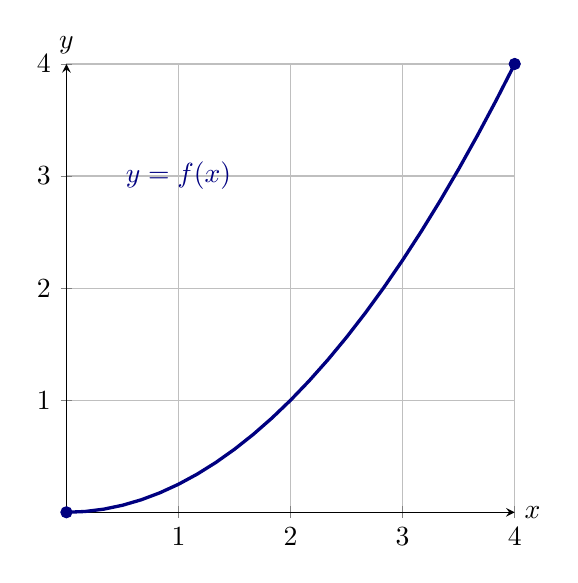
\begin{tikzpicture}
    \begin{axis}[
        xmin=0,xmax=4,ymin=0,ymax=4,
        clip=false,
        unit vector ratio*=1 1 1,
        axis lines=center,
        grid = major,
        ytick={-1,...,4},
	xtick={0,...,4},
        xlabel=$x$, ylabel=$y$,
        every axis y label/.style={at=(current axis.above origin),anchor=south},
        every axis x label/.style={at=(current axis.right of origin),anchor=west},
      ]
     
       \addplot[very thick,penColor,domain=0:4] {(1/4)*x^2};
      \addplot[color=penColor,fill=penColor,only marks,mark=*] coordinates{(0,0)};  %% closed hole  
        \addplot[color=penColor,fill=penColor,only marks,mark=*] coordinates{(4,4)};  %% closed hole  
      \node[penColor] at (axis cs:1,3) [penColor] {$y=f(x)$};
      \end{axis}`
  \end{tikzpicture}
  \end{image}

  Select  the correct statement.  
  \begin{hint}
  Recall, a function $g$ has to be continuous on a closed interval $[a,b]$ and differentiable on an open interval $(a,b)$, so that we can apply the Mean value theorem.
  If the above  conditions are satisfied, the the Mean value theorem (MVT) guarantees that there exists a point $c$ in $(a,b)$ such that $f'(c)=\frac{f(b)-f(a)}{b-a}$. 
    \end{hint}
\begin{selectAll}
\choice[correct]{The function $f$ satisfies the conditions of the MVT on its domain.}
\choice{The function $f$ does not satisfy the conditions of the MVT on its domain, because  $f$ is not continuous on its domain.}
\choice{The function $f$ does not satisfy the conditions of the MVT on its domain, because $f$ is not differentiable on $(0,4)$.}
\end{selectAll}
\end{exercise}
  \begin{exercise}
   \begin{image}
  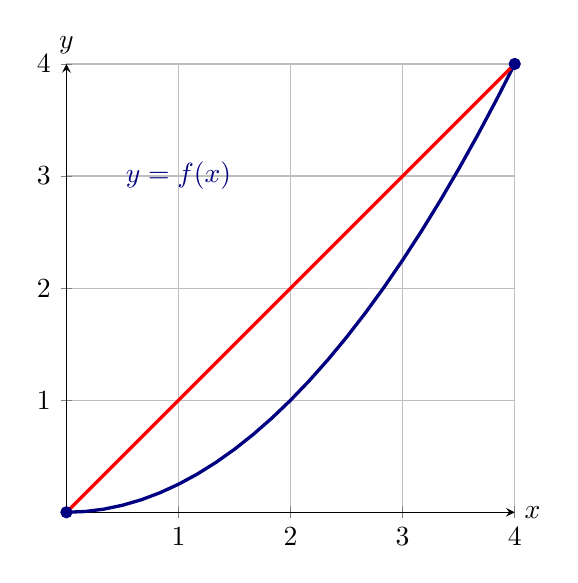
\begin{tikzpicture}
    \begin{axis}[
        xmin=0,xmax=4,ymin=0,ymax=4,
        clip=false,
        unit vector ratio*=1 1 1,
        axis lines=center,
        grid = major,
        ytick={-1,...,4},
	xtick={0,...,4},
        xlabel=$x$, ylabel=$y$,
        every axis y label/.style={at=(current axis.above origin),anchor=south},
        every axis x label/.style={at=(current axis.right of origin),anchor=west},
      ]
     
       \addplot[very thick,penColor,domain=0:4] {(1/4)*x^2};
      \addplot[very thick, color=red, smooth, domain=(0:4)] {x};
      \addplot[color=penColor,fill=penColor,only marks,mark=*] coordinates{(0,0)};  %% closed hole  
        \addplot[color=penColor,fill=penColor,only marks,mark=*] coordinates{(4,4)};  %% closed hole  
      \node[penColor] at (axis cs:1,3) [penColor] {$y=f(x)$};
      \end{axis}`
  \end{tikzpicture}
  \end{image}

 Let $m$ be the slope of the secant line through the points $(0,f(0))$ and $(4,f(4))$ (see figure above). Select the correct statement.
  
\begin{selectAll}
\choice{$m=4$}
\choice{$m=-4$}
\choice[correct]{$m=1$}
\choice{$m=-1$}
\choice{$m=0$}
\choice{$m=8$}
\choice{$m=-8$}
\choice{$m=2$}
\choice{$m=6$}
\choice{$m=8$}
\end{selectAll}
\end{exercise}
  \begin{exercise}
  Complete the statement below  regarding the function $f$ on the interval $[0,4]$.
  
  
 Select all correct choices.
 (Note, $m$, the slope of the secant line through the points $(0,f(0))$ and $(4,f(4))$, was computed in the previous exercise.)
 
 STATEMENT:
  
  The Mean value theorem guarantees that there exists a point $c$ in the open interval $(0,4)$ such that 
    \begin{selectAll}
\choice{$f'(c)=4$}
\choice{$f(c)=4$}
\choice{$f(c)=m$}
\choice[correct]{$f'(c)=m$}
\choice[correct]{$f'(c)=1$}
\choice{$f(c)=1$}
\choice{$f'(c)=-1$}
\choice{$f(c)=-1$}
\choice[correct]{$f'(c)=\frac{f(4)-f(0)}{4}$}
\choice{$f(c)=\frac{f(4)-f(0)}{4}$}
\end{selectAll}
\end{exercise}

 \begin{exercise}
Find a point $c$ in $(0,4)$, guaranteed by the MVT, such that

 $f'(c)=\frac{f(4)-f(0)}{4-0}$. Select the correct choice.
\begin{hint}
Observe the figure below. It shows that the \textbf{secant line} through the points $(0,f(0))$ and $(4,f(4))$ is \textbf{parallel} to the \textbf{tangent line} to the curve $y=f(x)$ at the point $x=\answer{2}$.
 \begin{image}
  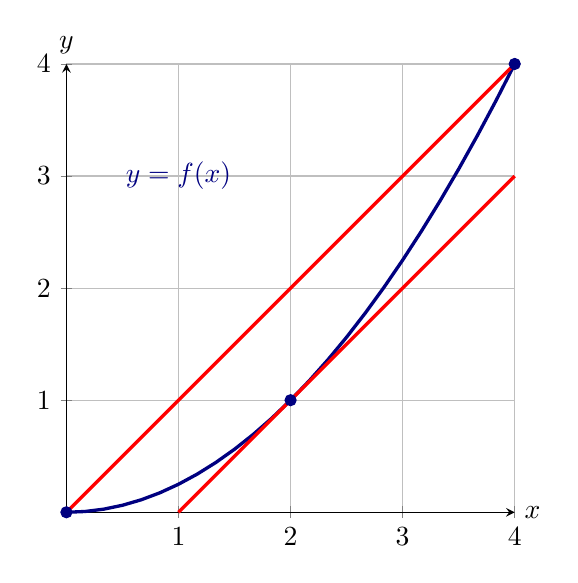
\begin{tikzpicture}
    \begin{axis}[
        xmin=0,xmax=4,ymin=0,ymax=4,
        clip=false,
        unit vector ratio*=1 1 1,
        axis lines=center,
        grid = major,
        ytick={-1,...,4},
	xtick={0,...,4},
        xlabel=$x$, ylabel=$y$,
        every axis y label/.style={at=(current axis.above origin),anchor=south},
        every axis x label/.style={at=(current axis.right of origin),anchor=west},
      ]
     
       \addplot[very thick,penColor,domain=0:4] {(1/4)*x^2};
      \addplot[very thick, color=red, smooth, domain=(0:4)] {x};
       \addplot[very thick, color=red, smooth, domain=(1:4)] {x-1};
      \addplot[color=penColor,fill=penColor,only marks,mark=*] coordinates{(0,0)};  %% closed hole  
        \addplot[color=penColor,fill=penColor,only marks,mark=*] coordinates{(2,1)};  %% closed hole  
        \addplot[color=penColor,fill=penColor,only marks,mark=*] coordinates{(4,4)};  %% closed hole  
      \node[penColor] at (axis cs:1,3) [penColor] {$y=f(x)$};
      \end{axis}`
  \end{tikzpicture}
  \end{image}
\end{hint}
\begin{selectAll}
\choice{$c=1$}
\choice[correct]{$c=2$}
\choice{$c=3$}
\choice{$c=4$}
\end{selectAll}

\end{exercise}
\begin{exercise}
 Find an equation of tangent line to the curve $y=f(x)$ at the point where $x=2$.
 \begin{hint}
 You have enough information to write an equation of a line: you know the coordinates of a point $(c,f(c)$ and the slope of the (tangent) line, $f'(c)$.
  \end{hint}
  Select all correct choices.
  
 
  \begin{selectAll}
\choice{$y=1$}
\choice{$y=2$}
\choice{$y=f'(x)$}
\choice{$y-2=1(x-1)$}
\choice{$y=x+1$}
\choice[correct]{$y-1=1(x-2)$}
\choice[correct]{$y=x-1$}
\choice{$y=f(x)$}
\end{selectAll}
\end{exercise}

\end{document}
